\documentclass[notitlepage,a4paper,11pt,hyperref=pdftex]{revtex4-1}
\usepackage{docs}
\usepackage[T2A]{fontenc}
\usepackage[utf8x]{inputenc}
% Русский язык
% \usepackage[english,russian]{babel}

% Математические сиволы 
\usepackage{amssymb,amsfonts,amsmath,mathtext}
\usepackage{textcomp}
% Гиперссылки
\usepackage[unicode, bookmarks=true,colorlinks,linkcolor=red,citecolor=green,urlcolor=blue]{hyperref}
\usepackage{bbold}

% Изображения
\usepackage[pdftex]{graphicx}

% Цвета
\usepackage[usenames]{color}
\usepackage{colortbl}


% Для квантовой физики
\renewcommand{\tan}{\mathop{\rm tg}\nolimits}
\newcommand{\bra}[1]{\langle#1|}
\newcommand{\ket}[1]{|#1\rangle}
\newcommand{\bracket}[2]{\langle#1|#2\rangle}
\newcommand{\mean}[1]{\langle#1\rangle}
\newcommand{\means}[1]{\langle#1\rangle_{sym}}
\newcommand{\Tr}[1]{\textbf{Tr}\{#1\}}
\newcommand{\dt}[1]{\frac{\partial #1}{\partial t}}
\newcommand{\I}[2]{\int\limits_{#1}^{#2}\,}

\usepackage{hhline}
\usepackage{lineno} % adding line number


% \linenumbers

% \ligodccnumber{T}{12}{000000}{}{v1}
% \ligodistribution{AIC, ISC}
\graphicspath{{images/}}
% \bibliographystyle{phaip}





% \author{Mikhail Korobko}

\begin{document}
\title{How to get analytical formula for filter?}
\maketitle
\begin{figure}
 \center{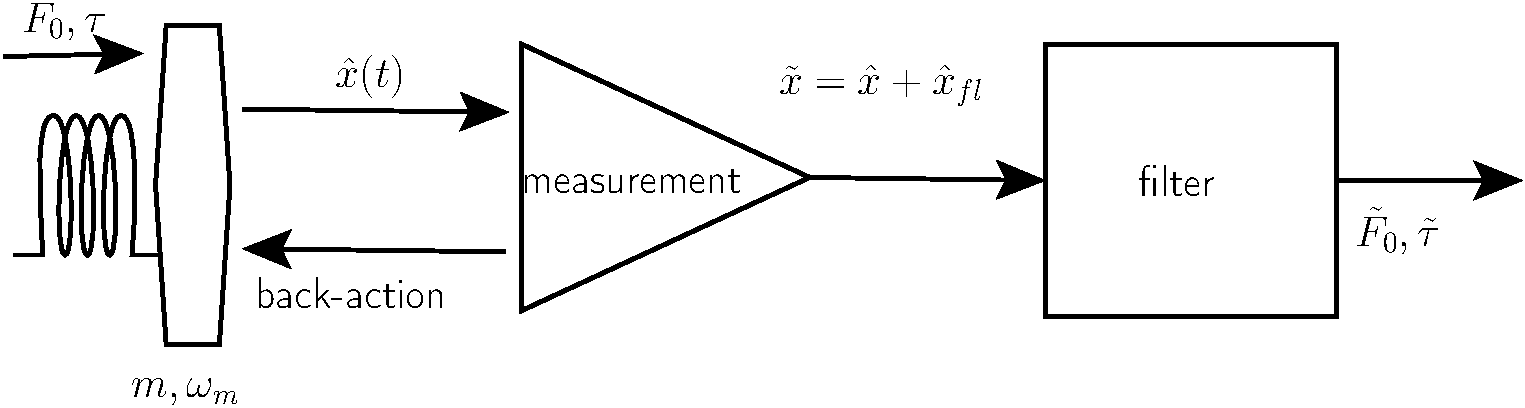
\includegraphics[width=0.8\textwidth]{measurement}}
\caption{General system}
\label{fig:meas}
\end{figure}

Let's consider simple case, without any particular measuring device (see Fig.\ref{fig:meas}). All we know about it is than it measures position of the oscillator and it has spectral densities of noises: $S_x,S_F, S_{xF}$
then we can calculate the optimal unbiased estimate minimizing the variation.

Our system is described by the following equation:
\begin{equation}
 \mathbf{D}\hat{x}(t) = m\ddot{\hat{x}}(t) + m \omega_m^2 \hat{x}(t) = F_s(t) + \hat{F}_{fl}(t), 
\end{equation}
where $F_s(t) = F_0\delta(t-\tau)$ is our signal force and we want to estimate it's amplitude $F_0$

We can write down the general solution for this equation:
\begin{equation}
 \hat{x}(t) = \hat{x}(0)\cos\omega_mt + \frac{\hat{p}(0)}{m\omega_m}\sin\omega_mt + \mathbf{D}^{-1}(F_s(t) + \hat{F}_{fl}(t))
\end{equation}
Here we notice, that $\hat{x}(t)$ is coordinate of the oscillator, and after measuring device it is $\tilde{x}(t) = \hat{x}(t)+\hat{x}_{fl}(t)$
Then we have to get rid of initial conditions. Normally it can be done by applying operator $\mathbf{D}$ to the output signal $\tilde{x}(t)$. But in this case we get 
\begin{equation}
 \tilde{F}(t) = \mathbf{D}\tilde{x}(t) = F_s(t) + \hat{F}_{fl}(t) + \mathbf{D}\hat{x}_{fl}(t)
\end{equation}
and we get the delta function with unknown parameter, that can't be linearized. More specifically, even if we apply the spectral approach here, we get:
\begin{equation}
 F_s(\omega) = \I{-\infty}{\infty}dt\,F_0\delta(t-\tau)e^{-\imath\omega t} = F_0 e^{-\imath\omega \tau}
\end{equation}
and we can't linearize it.

That's why we now can say just ``let's consider in insufficient'' and throw these terms:
\begin{multline}
 \tilde{x}(t) = \hat{x}_{fl}(t) + \frac{1}{m\omega_m}\I{0}{t}dt'\,(F_s(t') + \hat{F}_{fl}(t'))\sin\omega_m(t-t') =\\
= \hat{x}_{fl}(t) + \frac{1}{m\omega_m}(F_0\cos\omega_m\tau \sin\omega_mt - F_0\sin\omega_m\tau\cos\omega_mt) + \frac{1}{m\omega_m}\I{0}{t}dt'\,\hat{F}_{fl}(t')\sin\omega_m(t-t')
\end{multline}
or we can change $A_c = \frac{1}{m\omega_m}F_0\cos\omega_m\tau$ and $A_s = \frac{1}{m\omega_m}F_0\sin\omega_m\tau$ and get linear equation:
\begin{equation}
 \tilde{x}(t)=\hat{x}_{fl}(t) + A_c\sin\omega_mt - A_s\cos\omega_mt + \frac{1}{m\omega_m}\I{0}{t}dt'\,\hat{F}_{fl}(t')\sin\omega_m(t-t')
\end{equation}
then we proceed filtering:
\begin{equation}
 \begin{cases}
  \tilde{A}_c = \I{-\infty}{\infty}\,g_1(t')\tilde{x}(t')\,dt'\\
\tilde{A}_s = \I{-\infty}{\infty}\,g_2(t')\tilde{x}(t')\,dt'
 \end{cases}
\end{equation}
in order to get unbiased estimation, which means that $\tilde{A}_{c,s} = \bar{A}_{c,s} = A_{c,s}$, we should have constraints for the filtering functions:
\begin{align}
 \I{-\infty}{\infty}g_1(t')\sin\omega_mt'\,dt' =& 1\\
 \I{-\infty}{\infty}g_2(t')\cos\omega_mt'\,dt' =&1
\end{align}
Then for variations (we omit the formulas for $A_s$,because they are similar to that with $A_c$):
\begin{multline}
 \mean{(A_c-\tilde{A}_c)^2} = \I{-\infty}{\infty}dt\,g_1(t)\,\bigl(\mean{\hat{x}_{fl}^2} +\frac{1}{m^2\omega_m^2}\iint\limits_{0}^{t}dt'\,dt''\,\mean{F_{fl}(t'),F_{fl}(t'')}\sin\omega_m(t-t')\sin\omega_m(t-t'')+\\
+ \frac{2}{m\omega_m}\I{0}{t}dt'\,\mean{F_{fl}(t'),x_{fl}(t)}\sin\omega_m(t-t')\bigr) 
\end{multline}
We assume, that knowing spectral densities we can calculate correlation functions and all the big term inside parentheses in previous equation (let's call it $K(t)$):
\begin{equation}
 \mean{(A_c-\tilde{A}_c)^2} = \I{-\infty}{\infty}dt\,g_1(t)\,K(t)
\end{equation}
then we construct the Lagrange function:
\begin{equation}
 L[g_1(t)] = \I{-\infty}{\infty}dt\,g_1(t)\,K(t) + \lambda(\I{-\infty}{\infty}g_1(t')\sin\omega_mt'\,dt' -1)
\end{equation}
and variate it over $g_1$:
\begin{equation}
 \delta L[g_1(t)] = \I{-\infty}{\infty}dt(2g_1(t)\,K(t) + \lambda\sin\omega_mt)\delta g_1(t) = 0
\end{equation}
Then, using the main lemma of calculus of variations, we get:
\begin{equation}
\begin{cases}
 2 g_1(t)K(t) + \lambda\sin\omega_mt = 0\\
\I{-\infty}{\infty}g_1(t')\sin\omega_mt'\,dt' =1
\end{cases}
\end{equation}
 if we know the the $K(t)$ this system can be simply solved and we get the filtering function.

What is good about this approach: we have analytical formula for continuous case and we can calculate all variations and other stuff we want to.
What is bad: really huge formula, trowing the initial conditions.But nevertheless, the good thing is, that for simple case of 3 measurements we can calculate is and get some result.
\end{document}
